\documentclass{article}

\usepackage{fancyhdr}
\usepackage{extramarks}
\usepackage{amsmath}
\usepackage{amsthm}
\usepackage{amsfonts}
\usepackage{tikz}
\usepackage[plain]{algorithm}
\usepackage{algpseudocode}

\usetikzlibrary{automata,positioning}

\usepackage{graphicx}
\graphicspath{ {./images/} }

%
% Basic Document Settings
%

\topmargin=-0.45in
\evensidemargin=0in
\oddsidemargin=0in
\textwidth=6.5in
\textheight=9.0in
\headsep=0.25in

\linespread{1.1}

\pagestyle{fancy}
\lhead{Yousef Alaa Awad}
\chead{\hmwkClass\: \hmwkTitle}
\rhead{\firstxmark}
\lfoot{\lastxmark}
\cfoot{\thepage}

\renewcommand\headrulewidth{0.4pt}
\renewcommand\footrulewidth{0.4pt}

\setlength\parindent{0pt}

%
% Create Problem Sections
%

\setcounter{secnumdepth}{0}
\newcounter{partCounter}
\newcounter{homeworkProblemCounter}
\setcounter{homeworkProblemCounter}{1}

\newcommand{\hmwkTitle}{Homework\ \#5}
\newcommand{\hmwkClass}{Power Systems Economics}

%
% Title Page
%

\title{
    \vspace{2in}
    \textmd{\textbf{\hmwkClass:\ \hmwkTitle}}\\
    \normalsize\vspace{0.1in}
    \vspace{3in}
}

\author{Yousef Alaa Awad}

% Problems start here
\begin{document}

\maketitle
\pagebreak

\section{4.1}
\textbf{Given:} Cheapo Electrons is an electricity retailer. The table below shows theload that it forecast its consumers would use over a 6-hour period. Cheapo Electrons purchased in the forward market nd the power exchange exactly enough energy to cover this forecast. The table shows the average price that it paid for this energy for each hour. As one might expect, the actual consumption of its customers did not exactly match the load forecast and it had to purchase or sell the difference on the spot market and the prices nidicated. Assuming that Cheapo Electrons sells energy to its customers at a flat rate of 24.00\$/MWh, calculate the profit or loss that it made during this 6-hour period. What would the rate that it should have charged its customers to break even?
\begin{center}
	\begin{tabular}{||c|c|c|c|c|c|c||}
		\hline
		Period                & 1     & 2     & 3       & 4     & 5     & 6     \\
		\hline \hline
		Load Forecast (MWh)   & 120   & 230   & 310     & 240   & 135   & 110   \\
		\hline
		Average Cost (\$/MWh) & 22.50 & 24.50 & 29.30   & 25.20 & 23.10 & 21.90 \\
		\hline
		Actual Load (MWh)     & 110   & 225   & 330     & 250   & 125   & 105   \\
		\hline
		Spot Price (\$/MWh)   & 21.60 & 25.10 & 32.00   & 25.90 & 22.50 & 21.50 \\
		\hline
	\end{tabular}
\end{center}

\subsection{A) Calculate the profit or loss that Cheapo Electrons made during this 6-hour period.}
To calculate the total revenue we simply need to multiply the actual load amounts per hour by the rate of 24.00\$/MWh and then sum them all up as shown below:
$$ 110*24 + 225*24 + 330*24 + 250*24 + 125*24 + 105*24 = \$27,480.00 $$
After this, we simply need to calculate the total cost, of which is just difference between the actual load and forecasted load multiplied by that hours spot price (shown in the table below) and then add that to the multiplication of the forward cost and load forecasted produced amount:
\begin{center}
	\begin{tabular}{||c|c|c|c|c|c|c||}
		\hline
		Period                & 1    & 2    & 3    & 4    & 5    & 6    \\
		\hline \hline
		Load Forecast (MWh)   & 120  & 230  & 310  & 240  & 135  & 110  \\
		\hline
		Actual Load (MWh)     & 110  & 225  & 330  & 250  & 125  & 105  \\
		\hline
		\textbf{Difference} & \textbf{-10} & \textbf{-5} & \textbf{20} & \textbf{10} & \textbf{-10} & \textbf{-5} \\
		\hline \hline
		Spot Price (\$/MWh)   & 21.60 & 25.10 & 32.00   & 25.90 & 22.50 & 21.50 \\
		\hline
		\textbf{Spot Transaction (\$)} & \textbf{-216.00} & \textbf{-125.50} & \textbf{640.00} & \textbf{259.00} & \textbf{-225.00} & \textbf{-107.50} \\
		\hline \hline
		Load Forecast (MWh)   & 120  & 230  & 310  & 240  & 135  & 110  \\
		\hline
		Average Cost (\$/MWh) & 22.50 & 24.50 & 29.30 & 25.20 & 23.10 & 21.90 \\
		\hline
		\textbf{Forward Expense (\$)} & \textbf{2700.00} & \textbf{5635.00} & \textbf{9083.00} & \textbf{6048.00} & \textbf{3118.50} & \textbf{2409.00} \\
		\hline
	\end{tabular}
\end{center}
And now, when you add together all the expenses/transaction that had to occur (not the revenue, yet!), you get a total cost incurred of $\$29,218.50$. This therefore means that the total profit/loss will be the following:
$$ Profit = Revenue - Cost = 27,480.00 - 29,218.50 = \$-1,738.50 $$
Since the profit is negative this means that \textbf{Cheapo Electrons made a loss of \$1,738.50.}

\subsection{B) What is the rate that it should have charged to its customers to break even?}
To calculate the break even rate that Cheapo Electrons should have charged we simply divide the total cost by the total actual load over the 6-hour period, as shown below:
$$ \frac{29,218.50\$}{(110+225+330+250+125+105)\text{MWh}} = \frac{29,218.50\$}{1145\text{MWh}} = \textbf{25.52\$/\text{MWh}} $$

\pagebreak
\section{4.2}
\textbf{Given:} The input-output curve of a gas-fired generating unit is approximated by the following function: $$ H(P) = 120+9.3*P+0.0025*P^2\frac{\text{MJ}}{\text{h}} $$ This unit has a minimum stable generation of 200MW and a maximum output of 500MW. The cost of has is 1.20\$/MJ. Over a 6-hour period, the output of this unit is sold in a market for electrical energy at the prices shown in the table below.
\begin{center}
	\begin{tabular}{||c||c|c|c|c|c|c||}
		\hline
		Period         & 1    & 2  & 3  & 4    & 5  &  6 \\
		\hline
		Price (\$/MWh) & 12.5 & 10 & 13 & 13.5 & 15 & 11 \\
		\hline
	\end{tabular}
\end{center}
\subsection{A) Assuming that this unit is optimally dispatched, is initial on-line and cannot be shut down, calculate its operational profit or loss for this period.}
First we must create a Cost Function, C(P) via simply just using the input-output curve H(P) and multiplying it by the cost of gas:
$$ C(P) = H(P) * (\text{Gas Cost}) = (120+9.3*P + 0.0025*P^2)*(1.20) = 144 + 11.16*P + 0.003*P^2$$
After this, we can find the marginal cost by simply taking the derivative of the Cost Function with respect to the input power needed:
$$ MC(P) = \frac{dC(P)}{dP} = 11.16 + 0.006*P $$
After this, we also know that the optimal dispatch is simply where $ MC(P) = Market Price $, therefore the production amount is simply $ P = \frac{Market Price - 11.16}{0.006} $. And this function is, as always, subject to the upper and lower bounds of the unit's stable generation minimum and maximum. Those minimums and maximums of power generation therefore mean that the marginal cost at below 200 and above 500 are fixed like so:
\begin{itemize}
	\item Marginal Cost at Mimimum (P = 200): $MC(200) = 11.16+0.006*(200) = 12.36\$/MWh$.
	\item Marginal Cost at Maximum (P = 500): $MC(500) = 11.16+0.006*(500) = 14.16\$/MWh$.
\end{itemize}
NOW, with all of this information, we can collate it to the following table to show the final profit/loss that the unit will generate:
\begin{center}
	\begin{tabular}{||c||c|c|c|c|c||}
		\hline
		Period & Price (\$/MWh) & Output P (MW) & Revenue (\$) & Cost (\$) & Profit (\$) \\
		\hline \hline
		1      & 12.50          & 223.33        & 2791.67      & 2786.03   & 5.63        \\
		\hline
		2      & 10.00          & 200.00        & 2000.00      & 2496.00   & -496.00     \\
		\hline
		3      & 13.00          & 306.67        & 3986.67      & 3848.53   & 138.13      \\
		\hline
		4      & 13.50          & 390.00        & 5265.00      & 4952.70   & 312.30      \\
		\hline
		5      & 15.00          & 500.00        & 7500.00      & 6474.00   & 1026.00     \\
		\hline
		6      & 11.00          & 200.00        & 2200.00      & 2496.00   & -296.00     \\
		\hline
	\end{tabular}
\end{center}
This therefore means, after summing up all the profit values, that \textbf{the profit for the 6-hour period of the unit running is \$690.07.}

\subsection{Python Script Output Verification}
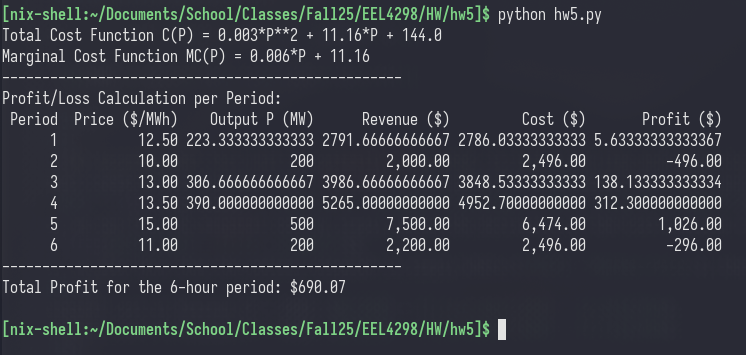
\includegraphics[width=\textwidth]{apple.png}

\end{document}
